\subsection{Problem 7}%
\label{sec:problem_7}

Draw the Gershgorin's disk, determine locations of the eigenvales for the matrices:
\begin{equation*}
    \matr{A_1} = 
    \begin{bmatrix}
        -2 & -1 &  0\\
         2 &  0 &  0\\
         0 &  0 &  2 
    \end{bmatrix},
    \matr{A_2} = 
    \begin{bmatrix}
        5 & 1 &  1\\
        0 & 6 &  1\\
        0 & 0 &  -5 
    \end{bmatrix},
    \matr{A_3} = 
    \begin{bmatrix}
        5.2 &  0.6 &  2.2\\
        0.6 &  6.4 &  0.5\\
        2.2 &  0.5 &  4.7 
    \end{bmatrix}
\end{equation*}
and estimate an upper bound for $cond(\matr{A}_i) : i = 1, \ldots, 3$.
Then, use any iteration methods to compute an approximate eigensystem.

\subsubsection*{Mathematics}
As stated in~\cite{Zdunek}, the Gershgorin circles may be used to define the bounds in
which the eigenvalues of a square matrix $\matr{A}\in\mathfrak{I}^{n\times{}n}$ are
located.

The Gershgorin circle is defined by:
\begin{equation}
    R_i(\matr{A}) = \{\lambda\in\mathfrak{I}:\lvert\lambda-a_{ii}\rvert\le\sum_{j\ne{}i}\lvert{}a_{ij}\rvert\}
\end{equation}
which means, that for each row $i$ of the matrix $\matr{A}$, we define a circle in the complex plane with
the center $c_i = a_{ii}$ and the radius $r_i = \sum_{j \neq i} |a_{ij}|$.
% https://mathoverflow.net/questions/350088/can-one-gershgorin-circle-only-contain-all-eigenvalues-when-the-other-circles
Starting with first matrix
\begin{equation*}
    \matr{A} = 
    \begin{bmatrix}
        -2 & -1 &  0\\
         2 &  0 &  0\\
         0 &  0 &  2 
    \end{bmatrix}
\end{equation*}
We define first circle center in:
\begin{equation*}
     c_1 = a_{11} = -2
\end{equation*}
Then we define disk radius
\begin{equation*}
    r_1 = \sum_{j \neq 1} |a_{1j}| = |a_{12}| + |a_{13}| = 1 
\end{equation*}
Then second:
\begin{equation*}
    c_2 = a_{22} = 0
    r_2 = \sum_{j \neq 2} |a_{2j}| = 2
\end{equation*}
And third row at last which doesn't have radius value
\begin{equation*}
    c_3 = a_{33} = 2
    r_3 = \sum_{j \neq 3} |a_{3j}| = 0
\end{equation*}
meaning that it's possible that one of eigenvalues would be equal to $\lambda_i = 2$.
Rest of problems and plots are in solution section.
%%%%%%%%%%%%%%%%%%%%%%%%%%%%%%%%%%%%%%%%%%%%%%%%%%%%%%%%%%%%%%%%%%%%%%%%%%%%%%%
\subsubsection*{Solution}
%%%%%%%%%%%%%%%%%%%%%%%%%%%%%%%%%%%%%%%%%%%%%%%%%%%%%%%%%%%%%%%%%%%%%%%%%%%%%%%
\begin{enumerate}
    \item matrix 
    
    \begin{equation*}
        \matr{A} = 
        \begin{bmatrix}
            -2 & -1 &  0\\
            2 &  0 &  0\\
            0 &  0 &  2 
        \end{bmatrix}
    \end{equation*}

    \begin{figure}[H]
        \centering
        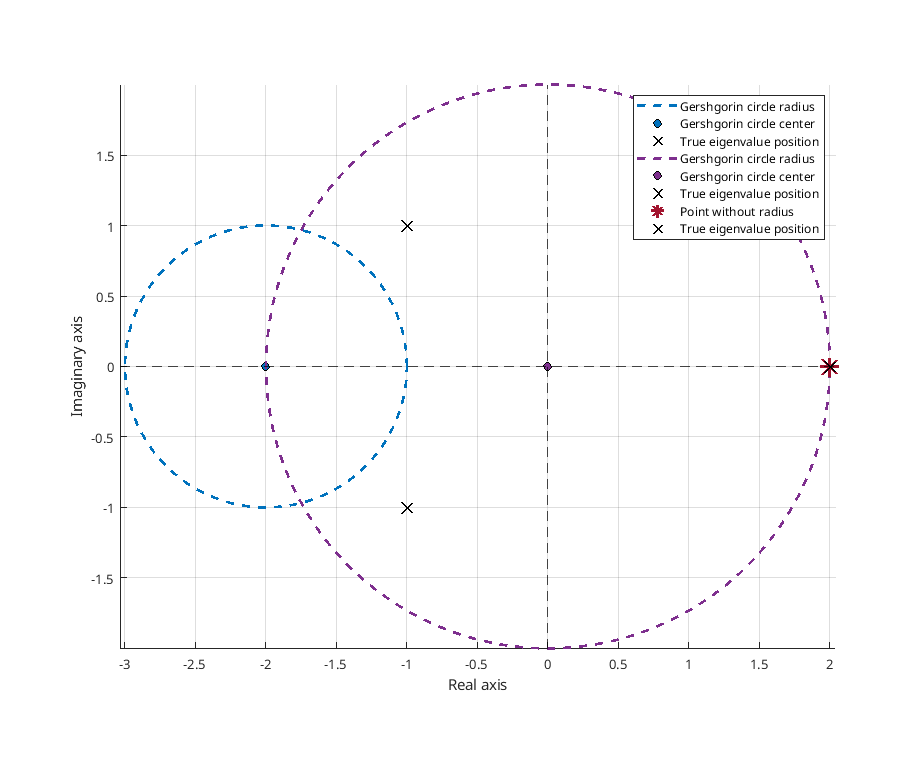
\includegraphics[width=1\textwidth]{problems/Figures/Problem_7/first_matrix.png}
        \caption{Gershgorin disks for first problem with true eigenvalues plotted.}
        \label{fig:Inverse}
    \end{figure}
    This matrix is specific case where one of gershgorin circles doesn't contain eigenvalue inside of it, its mostly because this matrix isn't diagonally dominant.
    \item matrix
    
    \begin{equation*}
        \matr{A} = 
        \begin{bmatrix}
            5 & 1 &  1\\
            0 & 6 &  1\\
            0 & 0 &  -5 
        \end{bmatrix}
    \end{equation*}

    \begin{figure}[H]
        \centering
        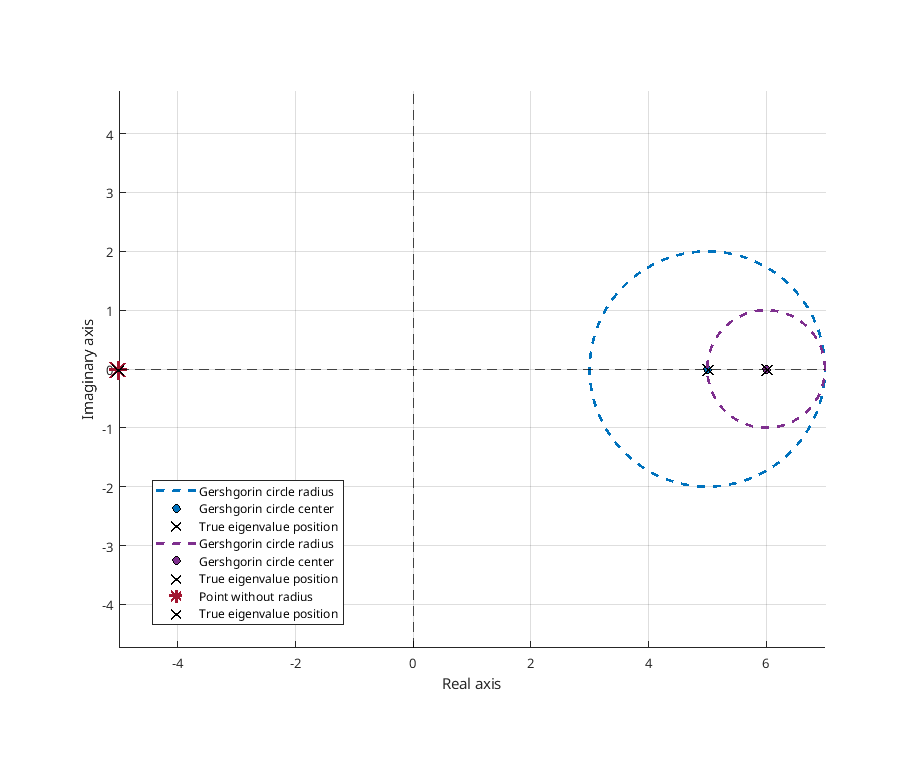
\includegraphics[width=1\textwidth]{problems/Figures/Problem_7/second_matrix.png}
        \caption{Gershgorin disks for second problem with true eigenvalues plotted}
        \label{fig:Inverse}
    \end{figure}
    \item matrix
    
    \begin{equation*}
        \matr{A} = 
        \begin{bmatrix}
            5.2 &  0.6 &  2.2\\
            0.6 &  6.4 &  0.5\\
            2.2 &  0.5 &  4.7 
        \end{bmatrix}
    \end{equation*}

    \begin{figure}[H]
        \centering
        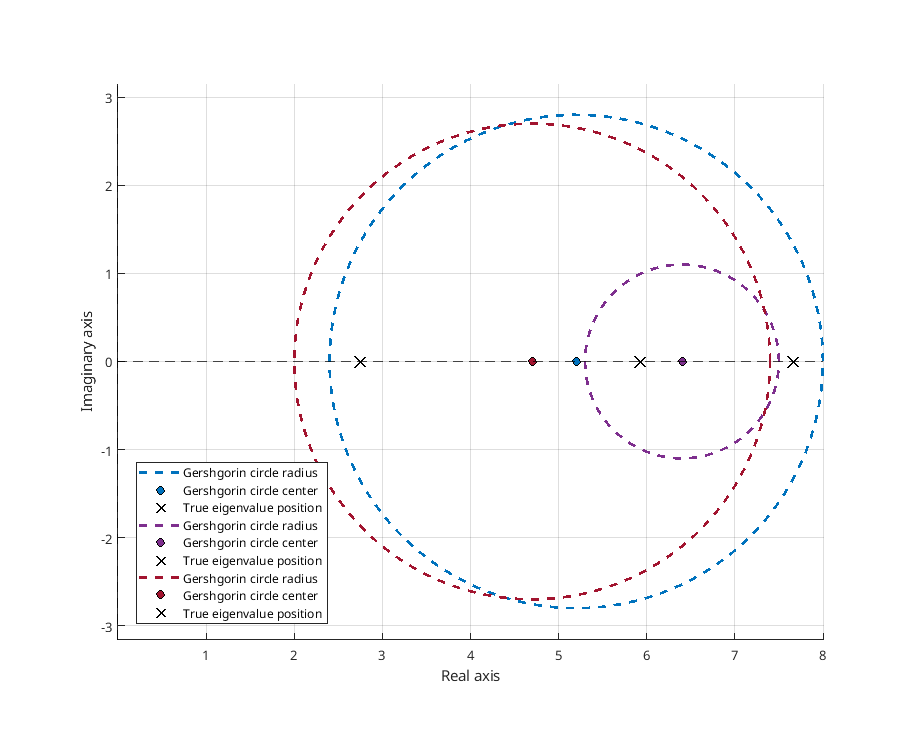
\includegraphics[width=1\textwidth]{problems/Figures/Problem_7/last_matrix.png}
        \caption{Gershgorin disks for last problem with true eigenvalues plotted}
        \label{fig:Inverse}
    \end{figure}
\end{enumerate}
